\subsection{Gaussian Elimination - Chapter 9 and 10}

\begin{enumerate}

\item {\bf Solving Multiple Algebraic Equations}

Solving multiple algebraic equations is very simple. For example if we
were to solve 

\begin{equation}
\begin{matrix} x + y = 2 \\
y-x = 4
\end{matrix}
\end{equation}

We would simply set $x=2-y$ and plug this into the equation below
yielding $y-(2-y)=4$ and thus $y=3$ and $x=-1$. It is also possible to
solve these equations graphically. If the first equation is written in
the form $y = 2-x$ and the second equation is written in the form $y =
4+x$ the solution to this system of equations is where the graphs
intersect. 

\begin{figure}[htb]
  \begin{center}
    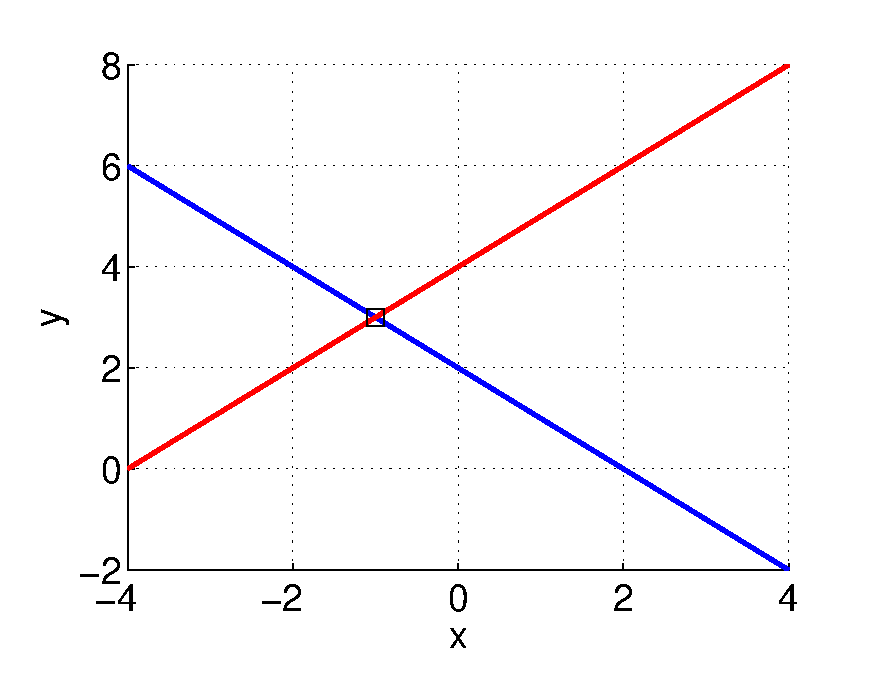
\includegraphics[height=0.5\textwidth,width=0.6\textwidth]{Graphics/Gaussian_Elimination}
  \end{center}
\end{figure}

However, it is also possible to take the first equation and add it to the second
equation. This would yield $2y=6$ and thus $y=3$. The second method is
known as Gaussian Elimination. This can be written in matrix form
using the equation below

\begin{equation}
\begin{bmatrix} 1 & 1 \\ -1 & 1 \end{bmatrix}
\begin{Bmatrix} x \\ y \end{Bmatrix} = 
\begin{Bmatrix} 2 \\ 4 \end{Bmatrix}
\end{equation}

This is the general form of $A\vec{x} = \vec{b}$. To use Gaussian
Elimination in Matrix form an augmented matrix is formed such that
$\tilde{A} = [A|b]$. This would yield the following equation.

\begin{equation}
\begin{bmatrix}
1 & 1 & 2 \\
-1 & 1 & 4
\end{bmatrix}
\end{equation}

Adding the first row to the second would yield

\begin{equation}
\begin{bmatrix}
1 & 1 & 2 \\
0 & 2 & 6
\end{bmatrix}
\end{equation}

Dividing the last equation by 2 would yield

\begin{equation}
\begin{bmatrix}
1 & 1 & 2 \\
0 & 1 & 3
\end{bmatrix}
\end{equation}

Finally, we take the bottom equation and subtract it from the
first. That would yield.

\begin{equation}
\begin{bmatrix}
1 & 0 & -1 \\
0 & 1 & 3
\end{bmatrix}
\end{equation}
The form above is known as reduced row echelon form. The first matrix
is the identity matrix and we can use it to directly solve for x and
y. Here it is clear that $x = -1$ and $y = 3$. 

\item {\bf Equations with No Solutions - The Matrix Determinant}

Note however that often times the equations have no solution. Take for
example the system. 
\begin{equation}
\begin{matrix} 2x + 2y = 1 \\
x+y = 1
\end{matrix}
\end{equation}
Using the ``Naive" Gaussian Elimination technique would yield the
following augmented matrix.
\begin{equation}
\begin{bmatrix}
2 & 2 & 1 \\
1 & 1 & 1
\end{bmatrix}
\end{equation}
The rref of the matrix above is then
\begin{equation}
\begin{bmatrix}
1 & 1 & 0.5 \\
0 & 0 & 0.5
\end{bmatrix}
\end{equation}
Notice here that the last row is all zeros. This doesn't make sense. 0
does not equal 0.5. In order to visualize what's happening we need to
look at this graphically. If we plot the first equation in the form
$y=(1-2x)/2$ and the second equation in the form $1-x$ we can see that
the lines below do not intersect. This is why the rref of the
augmented matrix produces a row of zeros. 
\begin{figure}[htb]
  \begin{center}
    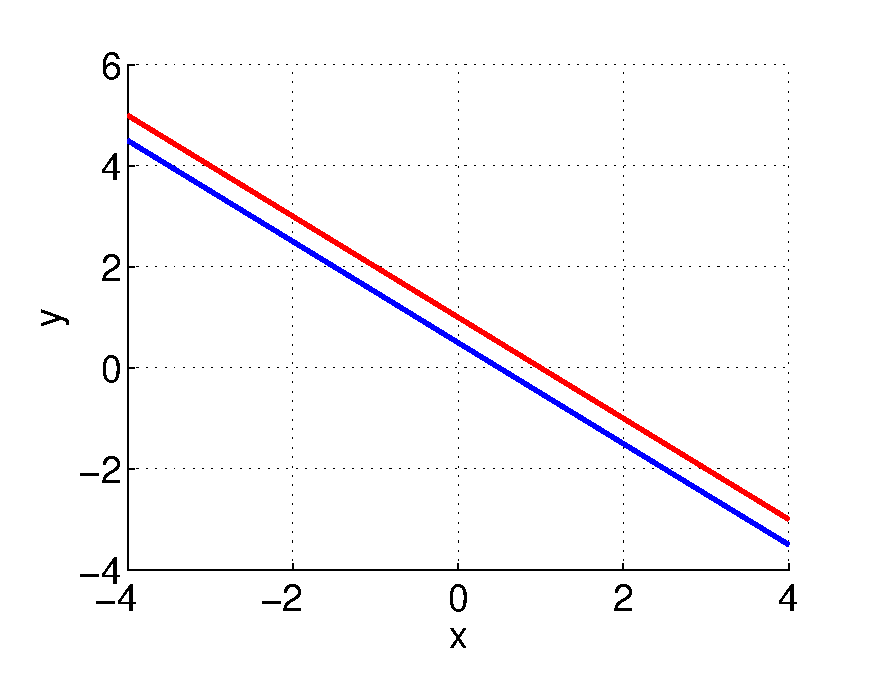
\includegraphics[height=0.5\textwidth,width=0.6\textwidth]{Graphics/No_Solution}
  \end{center}
\end{figure}
Rather than performing Gaussian Elimination it is sometimes useful to
compute the matrix determinant in order to see if a solution
exists. For a 2x2 matrix the determinant of a matrix is given by
\begin{equation}
det\begin{bmatrix} a & b \\ c & d \end{bmatrix} = ad-bc
\end{equation}
The determinant is a useful property because if the det = 0 the
solution does not exist and there will be a row of zeros in the rref
of the matrix. For example, let's take the first example where
\begin{equation}
A = \begin{bmatrix} 1 & 1 \\ -1 & 1 \end{bmatrix} 
\end{equation}
The det(A) is then simply 1*1-1*(-1) = 2 thus the solution
exists. However, if we take the second example
\begin{equation}
A = \begin{bmatrix} 2 & 2 \\ 1 & 1 \end{bmatrix} 
\end{equation}
the det(A) is 2*1-2*1 = 0 and thus the solution does not exist. This
can be helpful when doing systems of multiple variables like the
example below
\begin{equation}
\begin{bmatrix} 1 & 1 & 2\\ -1 & 1 & 3 \\ 2 & 4 & 5\end{bmatrix}
\begin{Bmatrix} x \\ y \\ z \end{Bmatrix} = 
\begin{Bmatrix} 2 \\ 4 \\ 5\end{Bmatrix}
\end{equation}
Using MATLAB we can write det(A) in the command window which returns
-8 which means the solution exists. Performing Gaussian elimination on
this problem yields
\begin{equation}
\begin{bmatrix} 1 & 0 & 0 & -0.3750 \\ 0 & 1 & 0 & -0.1250 \\ 0 & 0 &
  1 & 1.25 \end{bmatrix}
\end{equation}
We can graph this result rewriting each equation in the
form. $z=(2-x-y)/2$, $z=(4+x-y)/3$ and $z=(5-2x-4y)/5$. These are
equations of planes and are plotted in MATLAB below.
\begin{figure}[htb]
  \begin{center}
    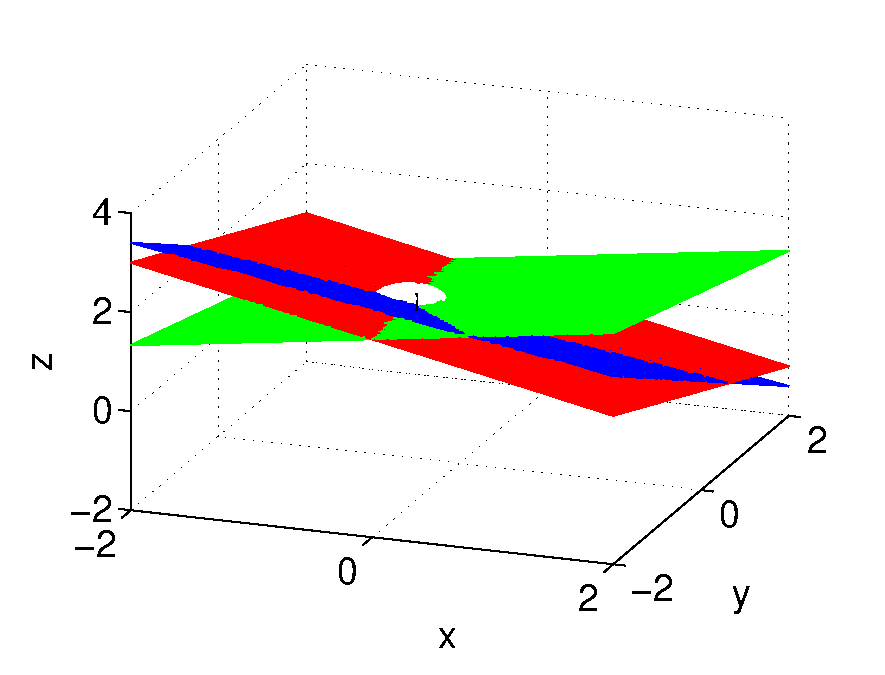
\includegraphics[height=0.5\textwidth,width=0.6\textwidth]{Graphics/Three_Planes}
  \end{center}
\end{figure}
The white ball is the intersection of all three planes and the
solution to the system of equations. If instead we take a look at the
system below.
\begin{equation}
\begin{bmatrix} 1 & 1 & 2\\ -2 & -2 & -4 \\ 2 & 4 & 5\end{bmatrix}
\begin{Bmatrix} x \\ y \\ z \end{Bmatrix} = 
\begin{Bmatrix} 2 \\ 4 \\ 5\end{Bmatrix}
\end{equation}
and compute det(A) in MATLAB the system returns 0 which means there is
no solution. This system can be plotted as well in MATLAB. 
\begin{figure}[htb]
  \begin{center}
    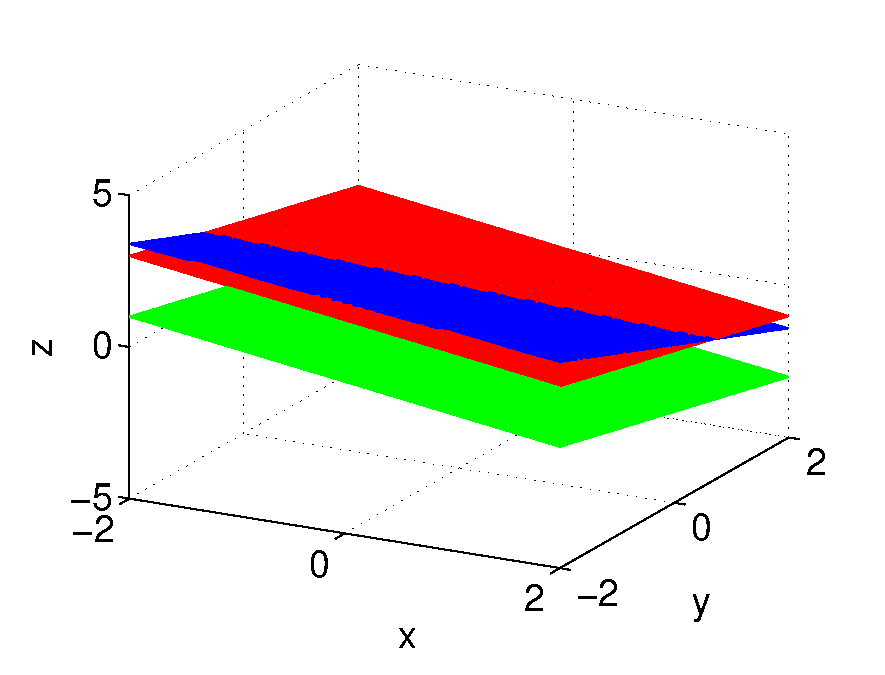
\includegraphics[height=0.5\textwidth,width=0.6\textwidth]{Graphics/No_Solution3}
  \end{center}
\end{figure}
Here it is clear that the red and green planes intersect however the
green plane is parallel to the red plane and thus there is no
solution. 

\item {\bf Eigenvalues($\lambda$) and Eigenvectors($\vec{\nu}$)}

Eigenvalues and Eigenvectors are used in a variety of different
applications including differential equations. Traditionally they are
used to solve problems of the form $A\vec{\nu}=\lambda\vec{\nu}$. In
order to solve these problems we subtract the right hand side to
achieve the form $(A-\lambda I)\vec{\nu}=0$. The solution is then
either $(A-\lambda I) = 0$ or $\vec{\nu} = 0$. However if the
eigenvector is equal to zero we obtain a trivial solution thus we
would like $(A-\lambda I)$ to be zero but it is impossible for this to
be true since the identity matrix is diagonal. Thus, the only way for
this solution to hold is for $det(A-\lambda I)=0$. The determinant is
a scalar equation and can be solved just like any other quadratic
equation. Using the eigenvalue it is possible to solve for the
eigenvector which is not unique but is typically normalized to
unity. As an example we will compute the eigenvalues of the matrix 
\begin{equation}
\begin{bmatrix}
1 & -2  \\
-2 & 1
\end{bmatrix}
\end{equation}
If we compute the determinant of this matrix we find that it is -3
which means the matrix has a solution if paired with a
vector. Computing $(A-\lambda I)$ yields
\begin{equation}
\begin{bmatrix}
1-\lambda & -2  \\
-2 & 1-\lambda
\end{bmatrix}
\end{equation}
The determinant is then simply $(1-\lambda)^2-4$. Solving this
equation is simply and yields two values, -1 and 3. Notice that the
determinant is the product of the eigenvalues. To find the
eigenvectors we then simply plug the eigenvalues into the matrix
$(A-\lambda I)$. This yields two matrix equations. 
\begin{equation}
\begin{bmatrix}
2 & -2  \\
-2 & 2
\end{bmatrix}\begin{Bmatrix}v_x \\ v_y\end{Bmatrix} = \begin{Bmatrix}
    0 \\ 0 \end{Bmatrix}
\end{equation}
If you notice, the determinant of the matrix is now zero thus the rref
is simply
\begin{equation}
\begin{bmatrix}
1 & -1  \\
0 & 0
\end{bmatrix}\begin{Bmatrix}v_x \\ v_y\end{Bmatrix} = \begin{Bmatrix}
    0 \\ 0 \end{Bmatrix}
\end{equation}
Thus we can pick any eigenvector $\vec{\nu} = [1,1]^T$. Doing the
same calculation for the eigenvalue of 3 yields an eigenvector of
$\vec{\nu} = [-1,1]^T$. If we normalize these vectors and place them
in matrix form we can write the eigenvector matrix as 
\begin{equation}
V = \begin{bmatrix} -0.7071 & -0.7071 \\ -0.7071 & 0.7071 \end{bmatrix} 
\end{equation}
The interesting property of this matrix is that it can be used to
decompose the matrix A into the form $A = V \Lambda V^{-1}$ where
\begin{equation}
\Lambda = \begin{bmatrix} \lambda_1 & 0 \\ 0 & \lambda_2 \end{bmatrix} = \begin{bmatrix} -1 & 0 \\ 0 & 3 \end{bmatrix} 
\end{equation}
This form is useful for the Matrix Inverse. The last thing to note is
that if the determinant of the matrix is zero it means on of the
eigenvalues is also zero. 

\item {\bf The Matrix Inverse}

The last way to solve equation is by using the matrix inverse. If the
equation is written in matrix form $A\vec{x} = \vec{b}$ the equation
can be multiplied by a special form of $A$ called the inverse such
that $A^{-1}A = I$ where $I$ is the identity matrix. The equation is
then $\vec{x} = A^{-1}\vec{b}$. For a 2x2 matrix the solution for the
matrix inverse is 
\begin{equation}
A^{-1} = \frac{1}{det(A)}\begin{bmatrix}b & -c \\ -d & a \end{bmatrix}
\end{equation}
Notice, that if det(A) is equal to zero the inverse does not
exist. This applies to all size matrices. However, for matrices with
bigger dimensions analytical solutions do not exist. Using the
augmented matrix it is possible to solve for the  
inverse of a matrix. For example. Let's assume we are trying to solve
for the inverse of the matrix.

\begin{equation}
\begin{bmatrix}
1 & 3  \\
4 & 2
\end{bmatrix}
\end{equation}

The augmented matrix to find an inverse involves putting the identity
matrix on the right-hand side such that $\tilde{A}=[A|I]$

\begin{equation}
\begin{bmatrix}
1 & 3 & 1 & 0\\
4 & 2 & 0 & 1
\end{bmatrix}
\end{equation}

With this augmented matrix Gaussian Elimination can be
performed. First the first row is multiplied by 4 and then substracted
from the second equation yielding
\begin{equation}
\begin{bmatrix}
4 & 12 & 4 & 0\\
0 & 10 & 4 & -1
\end{bmatrix}
\end{equation}
You can then divide the bottom equation by 10 and the top equation by
12.
\begin{equation}
\begin{bmatrix}
1/3 & 1 & 1/3 & 0\\
0 & 1 & 2/5 & -1/10
\end{bmatrix}
\end{equation}
Then subtract the second equation from the first and then multiply the
top equation by 3.
\begin{equation}
\begin{bmatrix}
1 & 0 & -1/5 & 3/10\\
0 & 1 & 2/5 & -1/10
\end{bmatrix}
\end{equation}
Thus our inverse is 
\begin{equation}
\begin{bmatrix}
-1/5 & 3/10\\
2/5 & -1/10
\end{bmatrix}
\end{equation}
Using this matrix you can solve any problem of the form
$A\vec{x}=\vec{b}$. For example,
\begin{equation}
\begin{bmatrix}
1 & 3  \\
4 & 2
\end{bmatrix}\begin{Bmatrix} x \\ y \end{Bmatrix} = \begin{Bmatrix} 1 
  \\ 1 \end{Bmatrix}
\end{equation}
The solution is then simply,
\begin{equation}
\begin{Bmatrix} x \\ y \end{Bmatrix} = \begin{bmatrix}
-1/5 & 3/10  \\
2/5 & -1/10
\end{bmatrix} \begin{Bmatrix} 1 \\ 1 \end{Bmatrix} = \begin{Bmatrix}
  1/10 \\ 3/10 \end{Bmatrix}
\end{equation}
We can also compute the rref of the augmented matrix to check the
solution.
\begin{equation}
rref(\begin{bmatrix}
1 & 3 & 1 \\
4 & 2 & 1
\end{bmatrix}) = \begin{bmatrix}
1 & 0 & 1/10 \\
0 & 1 & 3/10
\end{bmatrix}
\end{equation}
Finally, it is also possible to compute the inverse of the matrix
using the eigenvalue, eigenvector form. Remember the eigenvector,
eigenvalue form is $A=V \Lambda V^{-1}$. The interesting property about
the matrix V is that $V^{-1}=V^{-1}$. Thus $A^{-1} = V {\Lambda}^{-1}
V^{-1}$. The computation of $\Lambda^{-1}$ is trivial and can be done
using the equation below.
\begin{equation}
\Lambda^{-1} = \begin{bmatrix} \frac{1}{\lambda_1} & 0 \\ 0 & \frac{1}{\lambda_2} \end{bmatrix}
\end{equation}

\end{enumerate}



